%%%%%%%%%%%%%%%%%%%%%%%%%%%%%%%%%%%%%%%%%
% Jacobs Landscape Poster
% LaTeX Template
% Version 1.0 (29/03/13)
%
% Created by:
% Computational Physics and Biophysics Group, Jacobs University
% https://teamwork.jacobs-university.de:8443/confluence/display/CoPandBiG/LaTeX+Poster
% 
% Further modified by:
% Nathaniel Johnston (nathaniel@njohnston.ca)
%
% This template has been downloaded from:
% http://www.LaTeXTemplates.com
%
% License:
% CC BY-NC-SA 3.0 (http://creativecommons.org/licenses/by-nc-sa/3.0/)
%
%%%%%%%%%%%%%%%%%%%%%%%%%%%%%%%%%%%%%%%%%

%----------------------------------------------------------------------------------------
%	PACKAGES AND OTHER DOCUMENT CONFIGURATIONS
%----------------------------------------------------------------------------------------

\documentclass[final]{beamer}

\usepackage[scale=1.24]{beamerposter} % Use the beamerposter package for laying out the poster

\usetheme{confposter} % Use the confposter theme supplied with this template

\setbeamercolor{block title}{fg=white,bg=dblue!70} % Colors of the block titles
\setbeamercolor{block body}{fg=black,bg=white} % Colors of the body of blocks
\setbeamercolor{block alerted title}{fg=white,bg=dblue!70} % Colors of the highlighted block titles
\setbeamercolor{block alerted body}{fg=black,bg=dblue!10} % Colors of the body of highlighted blocks
% Many more colors are available for use in beamerthemeconfposter.sty

%-----------------------------------------------------------
% Define the column widths and overall poster size
% To set effective sepwid, onecolwid and twocolwid values, first choose how many columns you want and how much separation you want between columns
% In this template, the separation width chosen is 0.024 of the paper width and a 4-column layout
% onecolwid should therefore be (1-(# of columns+1)*sepwid)/# of columns e.g. (1-(4+1)*0.024)/4 = 0.22
% Set twocolwid to be (2*onecolwid)+sepwid = 0.464
% Set threecolwid to be (3*onecolwid)+2*sepwid = 0.708

\newlength{\sepwid}
\newlength{\onecolwid}
\newlength{\twocolwid}
\newlength{\threecolwid}
\setlength{\paperwidth}{48in} % A0 width: 46.8in
\setlength{\paperheight}{36in} % A0 height: 33.1in
\setlength{\sepwid}{0.024\paperwidth} % Separation width (white space) between columns
\setlength{\onecolwid}{0.30\paperwidth} % Width of one column
\setlength{\twocolwid}{0.624\paperwidth} % Width of two columns
\setlength{\threecolwid}{0.708\paperwidth} % Width of three columns
\setlength{\topmargin}{-0.5in} % Reduce the top margin size
%-----------------------------------------------------------

\usepackage{graphicx}  % Required for including images

\usepackage{booktabs} % Top and bottom rules for tables
\usepackage{exscale}


\usepackage{slivkins-setup,slivkins-theorems}

\newcommand{\term}[1]{\ensuremath{\mathtt{#1}}}

\def\varTheta{\bold{\Theta}}
\def\varOmega{\bold{\Omega}}
\def\ell{l}

% exploration sets
\newcommand{\AExp}{\mA} % actions
\newcommand{\MExp}{\mM}  % menus

% benchmarks
\def\OPT{\term{OPT}}
\newcommand{\OPTpub}{\OPT_{\term{pub}}}
\newcommand{\OPTpri}{\OPT_{\term{pri}}}
%----------------------------------------------------------------------------------------
%	TITLE SECTION 
%----------------------------------------------------------------------------------------

\title{Bayesian Exploration with Heterogeneous Agents} % Poster title

\author{Nicole Immorlica$^1$, Jieming Mao$^2$, Aleksandrs Slivkins$^1$, Zhiwei Steven Wu$^3$} % Author(s)

\institute{Microsoft Research$^1$, University of Pennsylvania$^2$, University of Minnesota$^3$} % Institution(s)

%----------------------------------------------------------------------------------------

\begin{document}

\addtobeamertemplate{block end}{}{\vspace*{2ex}} % White space under blocks
\addtobeamertemplate{block alerted end}{}{\vspace*{2ex}} % White space under highlighted (alert) blocks

\setlength{\belowcaptionskip}{2ex} % White space under figures
\setlength\belowdisplayshortskip{2ex} % White space under equations

\begin{frame}[t] % The whole poster is enclosed in one beamer frame

\begin{columns}[t] % The whole poster consists of three major columns, the second of which is split into two columns twice - the [t] option aligns each column's content to the top

\begin{column}{\sepwid}\end{column} % Empty spacer column

\begin{column}{\onecolwid} % The first column

%----------------------------------------------------------------------------------------
%	OBJECTIVES
%----------------------------------------------------------------------------------------

\begin{alertblock}{Problem}
\begin{itemize}
\item In recommendation systems, users both consume and produce information
\item Bayesian Exploration: a simple model which the recommendation system controls the information flow to users and strives to incentivize exploration via information asymmetry
\item We allow \emph{heterogeneous} users, relaxing a major assumption from prior work
\item Goal: learn the best \emph{personalized} recommendations
\end{itemize}
\end{alertblock}

%----------------------------------------------------------------------------------------
%	INTRODUCTION
%----------------------------------------------------------------------------------------

\begin{block}{Model}
~\\
A game consists of $T$ rounds between a principal and $T$ agents. Each round $t \in[T]$ proceeds as follows:
\begin{itemize}
\item Agent $t$ comes and its type $\theta_t$ is sampled
\item Agent $t$ receives message $m_t$ from the principal
\item Agent $t$ chooses action $a_t$
\item Agent $t$ obtains reward $r_t = u(\theta_t ,a_t, \omega)$ where $\omega$ is the ``state of nature'' sampled before the game starts. $r_t$ is revealed to the principal.
\end{itemize}
\textbf{Recommendation Policy $\pi$:} an algorithm decides how to send these messages $m_t$ adaptively\\
\textbf{Knowledge of types:} three model variants:
\begin{itemize}
\item public types: the type is revealed immediately after the agent arrives
\item reported types: the type is revealed only after the principal issues a recommendation
\item private types: the type is not revealed
\end{itemize}
\textbf{Bayesian Incentive Compatible (BIC):} for each agent $t$, following the suggested action in $m_t$ maximizing its expected reward\\
\textbf{``Revelation Principle'':} wlog consider restricted types of recommendation policies
\begin{itemize}
\item public types: $m_t$ is an action
\item reported/private types: $m_t$ is a menu mapping each state to an action
\end{itemize}
\end{block}


%------------------------------------------------

%\begin{figure}
%\includegraphics[width=0.8\linewidth]{MAB-2.jpg}
%\end{figure}

%----------------------------------------------------------------------------------------

\end{column} % End of the first column

\begin{column}{\sepwid}\end{column} % Empty spacer column

%\begin{column}{\twocolwid} % Begin a column which is two columns wide (column 2)


%----------------------------------------------------------------------------------------
%	IMPORTANT RESULT
%----------------------------------------------------------------------------------------

%\begin{alertblock}{aa}



%\end{alertblock} 

%----------------------------------------------------------------------------------------

\begin{columns}[t,totalwidth=\twocolwid] % Split up the two columns wide column again

\begin{column}{\onecolwid} % The first column within column 2 (column 2.1)

%----------------------------------------------------------------------------------------
%	MATHEMATICAL SECTION
%----------------------------------------------------------------------------------------

\begin{block}{Explorability and Benchmark}
~\\
\textbf{Explorability:} definition depends on model choices
\begin{itemize}
\item public types: \\
A type-action pair $(\theta, a)$ is called \emph{eventually-explorable} in state $\omega$ if there is some BIC recommendation policy can recommend this action to this agent type with positive probability\\
Use $\mathcal{A}_{\omega, \theta}$ to denote the set of all actions eventually-explorable for type $\theta$ and state $\omega$ 
\item private types: \\
A menu is called \emph{eventually-explorable} in state $\omega$ if there is some BIC recommendation policy can recommend this menu with positive probability\\
Use $\mathcal{M}_{\omega}$ to denote the set of all actions eventually-explorable for state $\omega$ 
\end{itemize}

\textbf{Benchmark:}
\begin{itemize}
\item public types:
\[
\OPTpub = \sum_{\theta \in \varTheta, \omega\in \varOmega} \Pr[\omega] \cdot \Pr[\theta] \cdot \max_{a \in \AExp_{\omega,\theta}} u(\theta, a, \omega)
\]
\item private types: 
\[
\OPTpri = \sum_{\omega\in \varOmega} \Pr[\omega] \cdot\max_{m \in \MExp_{\omega}}\sum_{\theta \in \varTheta} \Pr[\theta] \cdot  u(\theta, m(\theta), \omega)
\]
\end{itemize}
\end{block}

\begin{block}{Comparative Statics}
~\\
\textbf{Explorability and the Model Choice:} \\
Explorability is better in the public-type case compared to the private-type case.\\
Ex: 2 states, 2 types and 2 actions. States and types are drawn uniformly at random. Rewards are defined as follows:\\
	\begin{table}[H]
		\centering
		\begin{tabular}{|c||c|c|}
			\hline
			&$a=0$&$a=1$\\
			\hline
			\hline
			$\theta = 0$& $u = 3$ & $u =4$\\
			\hline
			$\theta = 1$& $u = 2$ & $u =0$\\
			\hline
		\end{tabular}
		\quad
		\begin{tabular}{|c||c|c|}
			\hline
			&$a=0$&$a=1$\\
			\hline
			\hline
			$\theta = 0$& $u = 2$ & $u =0$\\
			\hline
			$\theta = 1$& $u = 3$ & $u =4$\\
			\hline
		\end{tabular}
		\caption{Rewards $u(\theta,a,\omega)$ when $\omega =0 $ and $\omega = 1$.}
	\end{table}
\textbf{Explorability and Diversity:}
\begin{itemize}
\item public types: more types improve explorability
\item private types: more types may improve or hurt explorability 
\end{itemize}
\end{block}
%----------------------------------------------------------------------------------------

\end{column} % End of column 2.1

\begin{column}{\onecolwid} % The second column within column 2 (column 2.2)

%----------------------------------------------------------------------------------------
%	RESULTS
%----------------------------------------------------------------------------------------

\begin{block}{Recommendation Policy for Public Types}
~\\
\textbf{Thm:} Our recommendation policy gets total reward $(T- C)\cdot \OPTpub$ for some constant $C$ depends on the problem instance but not $T$\\
\begin{center}
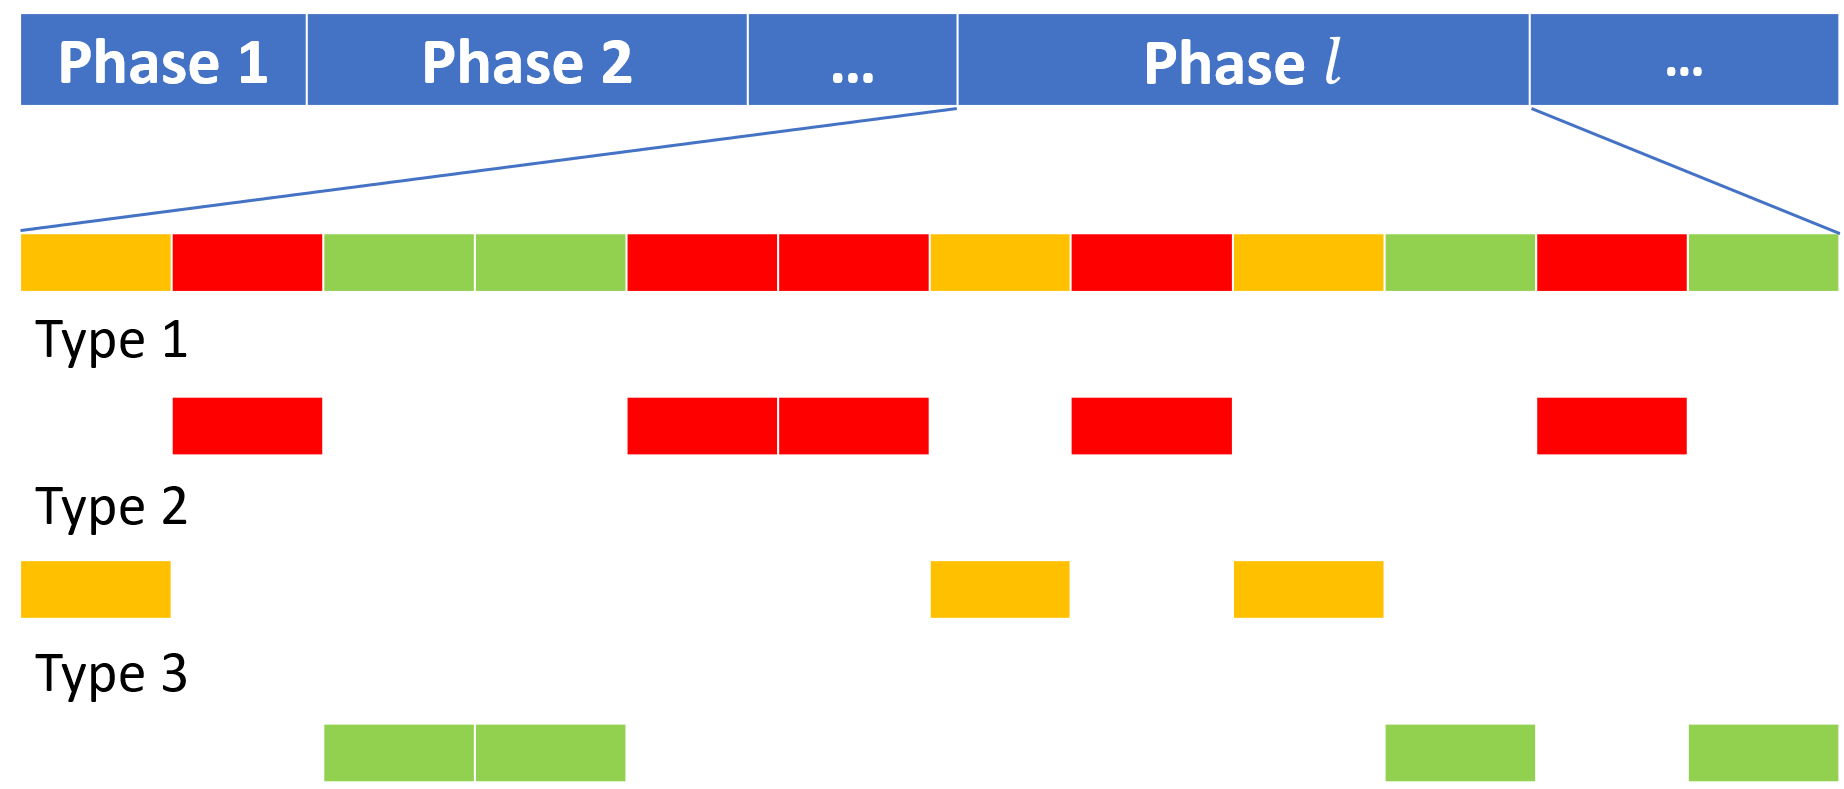
\includegraphics[width=0.99\linewidth]{recommendation.png} 
\end{center}

\textbf{Lemma:} The first $l$ phases of our recommendation policy explores all the action-type pair that is explorable by any BIC policy in $l$ rounds\\

\begin{itemize}
\item \textbf{Information Monotonicity:} Principal knowing more information won't hurt explorability \\

\item \textbf{Max-Support Policy:} Solve a linear program to find a single-round BIC policy that explores all the explorable actions with positive probabilities\\

\item \textbf{Maximal Exploration:} Turn the max-support policy into a sequence of actions that include all the explorable actions 
\end{itemize}
\end{block}

\begin{block}{Extension to Reported/Private Types}
~\\
\textbf{Reported Types:} simulate the public-type policy
\begin{itemize}
\item In each round $t$, guess agent type to be $\hat{\theta}_t$ 
\item Make progress if guess correctly 
\item Don't lose anything other than a round if guess incorrectly
\end{itemize}

\textbf{Private Types:} more complicated mainly because of the randomness of the types
\begin{itemize}
\item \textbf{Lemma:} The first $l$ phases of our recommendation policy explores all the menu that is explorable by any BIC policy in $l$ rounds \\
\item Try each menu many times
\item Approximate version of Information Monotonicity
\item Total reward $(T- C\log(T))\cdot \OPTpri$ 
\end{itemize}


\end{block}


%----------------------------------------------------------------------------------------

\end{column} % End of column 2.2

\end{columns} % End of the split of column 2

%\end{column} % End of the second column

\begin{column}{\sepwid}\end{column} % Empty spacer column

%\begin{column}{\onecolwid} % The third column

%----------------------------------------------------------------------------------------
%	CONCLUSION
%----------------------------------------------------------------------------------------

%----------------------------------------------------------------------------------------
%	ADDITIONAL INFORMATION
%----------------------------------------------------------------------------------------
%\begin{block}{aa}

%\end{block}

%\begin{block}{Future Directions}

%\end{block}
%----------------------------------------------------------------------------------------
%	REFERENCES
%----------------------------------------------------------------------------------------

%----------------------------------------------------------------------------------------
%	ACKNOWLEDGEMENTS
%----------------------------------------------------------------------------------------

%\setbeamercolor{block title}{fg=red,bg=white} % Change the block title color

%\begin{block}{Acknowledgements}

%\small{\rmfamily{aa.}} \\

%\end{block}


\setbeamercolor{block alerted title}{fg=black,bg=norange} % Change the alert block title colors
\setbeamercolor{block alerted body}{fg=black,bg=white} % Change the alert block body colors

%\begin{center}
%\includegraphics[width=0.4\linewidth]{Princeton_logo_svg.png} 
%\end{center}

%----------------------------------------------------------------------------------------

%\end{column} % End of the third column

\end{columns} % End of all the columns in the poster

\end{frame} % End of the enclosing frame

\end{document}
